\documentclass{article}

\usepackage{amsmath,amssymb}
\usepackage{mathrsfs}
\usepackage{braket}
\usepackage{graphicx}

\title{Connecting Particle and Field Mechanics}
\author{Anthony Mezzacappa}
\date{September 1 and 3, 2020}

\begin{document}

\setlength{\parskip}{1em}

\maketitle

\noindent Consider we have a classical linear chain of equal masses connected by spring of equal spring constant. The springs can oscillate about there equilibrium position in one dimension. In equilibrium all masses are separated by an equal length. \par

$\kappa$ = value of the spring constant \par
$a$ = length between the masses in equilibrium\par
$m$ = mass of each of the sampled masses\par

\begin{figure}[h!]
    \centering
    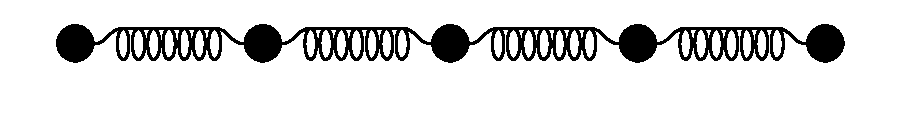
\includegraphics[width=\textwidth]{pics/04-linear-chain.pdf}
    \label{fig:l4-linear-chain}
\end{figure}

\noindent Define \par
\noindent $q_n(t) $= displacement of each oscillator from its equilibrium position $\bar{q}_n \equiv na $ i.e., $x_n(t) = na+q_n(t)$ \par
\noindent For simplicity, we will assume periodicity i.e., $q_1(t) =q_{N+1}(t)$ \par
\noindent In the limit $N \rightarrow \infty$, this will not matter. \par

% Page 2

\noindent The Lagrangian of this system is
\begin{equation}
    L = T - V  = \frac{1}{2} m \sum_{n=1}^N \dot{q}_n^2 - \frac{1}{2} \kappa \sum_{n=1}^N (q_{n+1} - q_n)^2
\end{equation}

\noindent It's only the difference in the displacements of the masses from their equilibrium position that contributes to the potential energy
\begin{align*}
    \left( x_{n+1} (t) - x_n (t) \right) - a &= ( n + 1 ) a + q_{n+1} (t) - n a - q_n (t) - a 
    &= q_{n+1} (t) - q_n (t)
\end{align*}

\noindent The Euler-Lagrangian EOM for each mass are
\begin{equation}
    \dfrac{ \partial L }{ \partial q_n} -  \dfrac{d}{ \mathrm{d} t} \left[\dfrac{ \partial L }{ \partial \dot {q}_n } \right] = 0
\end{equation}

$\dfrac{ \partial L }{ \partial q_n}$ :






\end{document}